\chapter{Applied Cryptography}%
\label{cha:Applied Cryptography}

\section{Introduction}
\begin{parag}{Why cryptography matters?}
    A lot of data need to move from one place to another while wanting to stay private (i.e. no one can stole the data during the trip). But not only, even data at rest (e.g. your password in your os) need also to not be accessible by a third party. To ensure this, one need to \important{encrypt} data.
\end{parag}
\begin{parag}{What can we do with cryptography}
    Cryptography is also the building block for:
	\begin{itemize}
	    \item \important{Integrity}: Ensuring data hasn't been tampered with (Hashing/Signatures)
	    \item \important{Authentication}: Verifying identity (Protocols)
		\item But also \important{Anonymity}, etc.
	\end{itemize}
	In this first lecture we will focus on the basics of using cryptography for confidentiality
\end{parag}

\subsection{The Core Problem For Today}
The central problem here is to \important{secure communication over an insecure channel}. We need a way for Alice to send a message to Bob, so that Eve (the adversary) cannot read it even though Eve have access to the channel where the massing is passing. 
\begin{framedremark}
confidentiality for data at rest can be seen as a particular case, where Alice $= $ Bob.
\end{framedremark}

\subsection{The origins of cryptography: the quest for confidentiality}
Before going into cryptography, let us first define what are we trying to ensure 
\begin{definition}{confidentiality : }
information cannot be accessed by unauthorized parties
\end{definition}
\begin{center}
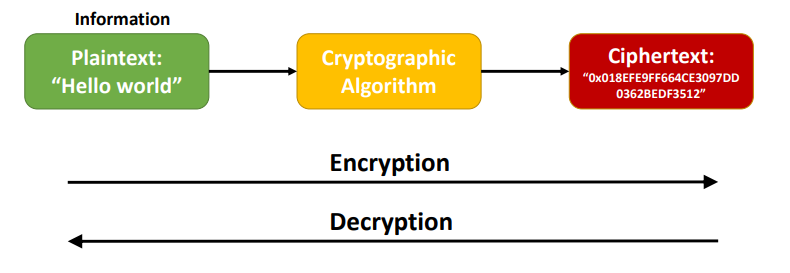
\includegraphics[scale=0.4]{screenshots/2026-10-10.png}
\end{center}
The goal is that the \important{encryption} cannot be reversed without the use of the \important{key}.
\begin{parag}{Cryptography as Functions}
    To have a more formal view of cryptography and being able to ensure confidentiality by proving it mathematically, let us define the encryption/decryption using functions. Here one should define
	\begin{itemize}
	    \item \important{Plaintext} $M$: Original message.
	    \item \important{Key}: $K$ Secret value.
	    \item \important{Ciphertext}: $C$ Scrambled message.
	\end{itemize}
	We then have the following equality 
	\begin{align*} 
		C &= E_K\left(M\right)\\
		M &= D_K\left(C\right)
	\end{align*}
\end{parag}
\begin{parag}{Cryptographic algorithms for confidentiality}
    In order to have confidentiality between Alice and Bob, both needs to either encrypt or decrypt the given message that the other is sending, to do so as seen in the equations above, both Alice and Bob need to share the same key $K$. Having a shared key between Alice and Bob, the algorithm works as follow
	\begin{itemize}
	    \item Encrypt message $m \to \text{Enc}\left(K, M\right)$
	    \item Send encrypted message $\text{Enc}\left(K, M\right) = c$
	    \item Decrypt message $c \to m = \text{Dec}\left(K, c\right)$
	\end{itemize}
	
\end{parag}
\begin{parag}{The core requirement --- Invertibility}
    An statement that we need to make in order to make the encryption/decryption mechanism works is that the decryption function $D_K$ must be the \important{invert} of $E_K$ :
	\begin{align*} 
		\forall K, M, D_K\left(E_K\left(M\right)\right) = M 
	\end{align*}
	If not, Bob cannot recover the original message $M$.
	\begin{framedremark}
	\important{Security requirement}: To provide security, these function must also be \important{hard to invert} without knowing the key $K$. If inverting a given function could be find meaning for instance that if we knew that the function for encryption was $e^{x}$, then it become quite easy to reverse it $\ln\left(c\right) = m$.
	\end{framedremark}
\end{parag}
\begin{parag}{Hard to invert: The Key Space}
    What we mean concretely when saying hard to invert is the following: To find the plaintext $M$, in an ideal cryptosystem, the only viable attack for the adversary (Eve) must be to try every single possible secret key $K$ (a \important{brute force attack})
\end{parag}

\begin{parag}{Example 1: Caesar's Cipher}
    The idea here is simple, we shift every later of the attack by a given number $K$, the key. The algorithm works as follow 
	\begin{itemize}
	    \item \important{Encryption}: Shift each letter by a fixed number $K$
	    \item \important{Decryption}: Shift each letter by a fixed number $-K$
	    \item \important{Key Space}: Only 25 possible keys.
	\end{itemize}
	If for instance the plaintext is \texttt{ATTACK AT DAWN}, the result Ciphertext is \texttt{DWWDFN DW GDZQ}.\\
	$ $\\
	\important{Security Insight}: $\log_2 \left(25\right) \approx 4.6$ bits of security. This is \important{far to small} for real-worls use.
	\begin{framedremark}
	The unit of measure use here $\log_2$ is called the '\textit{bits of security}' which is a logarithmic unit of measurement tat quantifies the \important{amount of computational effort required to break a cryptographic system}. If a system has $n$ bits of security, it means an attacker must perform roughly $2^{n}$ operations (or mathematical steps) to crack it using the best known attack.
	\end{framedremark}
\end{parag}
\begin{parag}{Cryptanalysis: The Flaw}
    \begin{itemize}
        \item Eve knows that Alice wrote a long-enough message for Bob in English.
        \item She knows that English most frequent letter is '\textit{e}'.
        \item She can then simply identify the most frequent letter in the ciphertext: it likely corresponds to the letter '\textit{e}'.
        \item She can then directly recover the key (a number between 0 and 25). This is a \important{frequency analysis attack}.
    \end{itemize}
\end{parag}
\begin{parag}{More than 25 keys: The substitutions Cipher}
	Here you could think, okay then I will just use more letter like $1000$ letters instead of $25$ and then my code is secure. To do so, one can use the substitution Cipher. In this case each letter is mapped to a unique, different letter defined by a \important{permutation} of the 26 letters. What this gives us is a key space of $26! \approx 4.03 \cdot 10^{26}$. $\log_2\left(26!\right) \approx 88.4$ bits of security?\\
	$ $\\
	However this cipher can still easily be broken using the same frequency analysis as before.
\end{parag}
\begin{parag}{Cryptanalysis: The Flaw, Again}
	\begin{itemize}
    	\item The same \important{frequency analysis attack} is effective against the Substitutions Cipher.
    	\item \important{Vulenrability}: The cipher preserves the statistical properties of the plaintext language (e.g., single-letter frequencies).
    	\item If Eve (the attacker) has a long enough ciphertext $C$, statistical analysis will break the cipher, rendering the full $26!$ key space \important{irrelevant}.
    	\item \important{Goal of the adversary}: Notice that the goal of the adversary might not be necessarily to recover the full key depending on the scenario, it might only attempt to recover part of the key (the mapping of a subset of letters) .
    	\item Sometimes the goal of the attacker is even smaller: Eve might want only to know wheter Alice sent the message '\textit{Yes}' or '\textit{No}' to Bob.
	\end{itemize}
\end{parag}

\begin{parag}{Bits of security verus Key Space Size}
    The goal that we would like to reach is that an $N$-bit key should offer security as close to $N$ bits as possible (i.e. require $2^{N}$ attempts). If a 1024-bit key is broken with '\textit{only}' $2^{40}$ attempts (40 bits of security), the algorithm is considered broken. However as seen in the Caesar, having a bigger key is not always a sign better, we also need to take into account that the adversaries are smart.
\end{parag}

\section{Adversaries in Cryptography}
\begin{parag}{Eve's Power: Passive Eavesdropping}
    In Caesar's (and the substitution) Cipher, eve's capabilities were very limited, she was only able to overse a long-enough ciphertext $C$ that corresponds to the encryption of a piece of English (and some compute power to test a few keys). Here this is kind of the lowest possible type of adversaries meaning an adversary with lower rights than this can pretty much do nothing. So let us see other possible adversary models
\end{parag}
\begin{parag}{Other Security Models: Type of Adversaries}
    As seen before, security is a schema that is always measured relative to the power of the \important{adversary (Eve)}
	\begin{itemize}
	    \item \important{Passive Eavesdropper}: Eve can only read the ciphertext
	    \item \important{More Active Attacker}: Eve can somehow influence the system by for example convincing Alice to send to Bob very specific messages, observing the precise time it takes Bob tu run its algorithm, etc... anything that can go beyond just observing the communication.
	\end{itemize}
\end{parag}
\begin{parag}{Active Model 1: Known Plaintext Attack (KPA)}
    The scenario is the following, Eve is given access to multiple pairs $\left(M, C\right)$ corresponding to messages and their corresponding ciphertext, all encrypted with the secret key $K$.\\
	$ $\\
	The goal is to go from this pairs to try to guess the key $K$ in order to decrypt other messages.
	\begin{subparag}{Why is KPA a Realistic Model?}
	    \begin{itemize}
	        \item \important{Standard Headers}: Many encrypted messages contain predictable headers (e.g. '\textit{from:}', or as in the film \textit{The Imitation Game})
	        \item \important{Malicious Guessing}: If Eve guesses a message (or a part of a message) and observes its encryption, she as an $M/C$ pair.
	    \end{itemize}
	\end{subparag}
	\begin{subparag}{KPA and the Substitutions Cipher}
	    If we know take the KPA model trying to attack the substitution cipher, it become even easier to crack it. Imagine that Eve knows that $M =  \text{'THE QUICK BROWN FOX'}$, she immediately recovers the mapping for multiple letters, drastically reducing the effective key space, without even needing to do statistical analysis study.
	\end{subparag}
\end{parag}

\begin{parag}{Active Model 2: Chosen Plaintext Attack (CPA)}
    The scenario is the following: Eve can somehow convince Alice (or the system) to encrypt arbitrary messages (chosen by Eve) with the secret key. More abstractly, for any chosen plaintext $m$, Eve can get access to $E_K\left(m\right)$.
	\begin{framedremark}
	We often say that Eve is assumed to have access to an \important{Encryption Oracle}.
	\end{framedremark}
	\begin{subparag}{Why is CPA a realistic model?}
	    We can imagine two simple scenarios 
		\begin{itemize}
		    \item \important{Alternative Scenario}: Think of a secure messaging service (like Signal  or WhatsApp) that uses the sender's key to encrypt the message. If Eve gets limited access to Alice's phone for a few minuts, she can maybe send any piece of data she choose to Bob, to generate an $\left(M, C\right)$ pair.
		    \item \important{Encryption API}: Eve might interact with an encrypted API endpoint where she provides data and receives the encrypted output.
		\end{itemize}
	\end{subparag}
	\begin{subparag}{CPA and the Substitution Cipher}
	    Here it is easy to show that the substitution cipher is completely broken by CPA as the attacker only have to ask for the encryption of the alphabet.
	\end{subparag}
\end{parag}

\begin{parag}{Practical Threat Model: Side-Channel Attacks}
    The scenario is the following: Eve is allowed to not only access an ideal oracle, but also
measure physical characteristics of the actual implementation while it
is encrypting/decrypting. This allows to have two new attacks:
\begin{itemize}
    \item \textbf{Timing Attack}:  Eve measures how long it takes for a given message to
get encrypted or a ciphertext to be decrypted.
	\item \textbf{Power Analysis}: Eve observes the energy consumed by the device
(e.g., a credit card) doing the crypto.
\end{itemize}

	\begin{subparag}{Why are Side-Channel a Realistic Model?}
	    \begin{itemize}
	        \item \textbf{Malicious Ownership}: ou often own a device (like a phone, smart card, or embedded chip) that holds keys belonging to another principal (e.g., Google, your bank) that are meant to be unreadable to you.
	        \item \textbf{Concrete Example (DRM)}: The decryption key for Digital Rights Management (DRM) content (like a movie or song) is embedded in your media player or console. By measuring power or timing signals, an attacker could potentially extract that secret key.
	    \end{itemize}
	    
	\end{subparag}
\end{parag}






\section{Perfect Secrecy and One-Time-Pad}


\begin{parag}{One-Time-Pad}
    The key is defined as a string $k$ of \important{random} bits \important{as long as the message}. Then one define the encrypted as 
	\begin{align*} 
		\text{Enc}\left(k, m\right) = m \oplus k 
	\end{align*}
	Here we that OTP  is \important{perfectly secure}.
	\begin{itemize}
	    \item For any ciphertext $C$, \important{every possible $M$ is equally likely}
	    \item The key $k$ is uniformly random, so $C$ gives the adversary \important{zero new information} about $M$.
	\end{itemize}
	\begin{definition}{Perfect Secrecy}
	To achieve perfect secrecy for a given encryption algorithm we need the follwing 
	\begin{align*} 
		\forall m, c, P\left(M = m | E_{K}\left(m\right) = c\right) = P\left(M = m\right) 
	\end{align*}
	Which means that for all message and their ciphertext, the probability of a plaintext $M$ being the message knowing the encryption is the same as the probability of the plaintext $M$ being the message.
	\end{definition}
	\begin{theoreme}
	One-Time-Pad achieves perfect secrecy
	\end{theoreme}
	\begin{proof}
	    To do so let us work through the LHS, we use that fact that $m \oplus K =  c \implies K = c \oplus m$ :
		\begin{align*} 
			P\left(M = m | E_K\left(m\right) = c\right) &= \frac{P\left(M = m \cap E_K\left(m\right) = c\right)}{P\left(E_K\left(m\right) = c\right)}  \\
														&= \frac{P\left(M = m \cap \left(m \oplus K\right) = c\right)}{P\left(E_k\left(m\right) = c\right)}\\
														&= \frac{P\left(M = m \cap K = m \oplus c\right)}{P\left(K =  m \oplus c\right)}\\
														&=  \frac{P\left(M = m\right) \cdot  P\left(K =  m \oplus c\right)}{P\left(K = m \oplus c\right)} = P\left(M = m\right)
		\end{align*}
	\end{proof}
	
	
\end{parag}
\begin{parag}{The Key Problem of OTP}
    OTP requires keys that are \important{truly random}, \important{message-length}, and \important{used only once}. And as securely pre-distributing message-length keys for real-world applications is impractical, OTP is not practical for real-world applications.
\end{parag}
\begin{parag}{Cryptanalysis Question: Key Reuse}
    Suppose Alice reuses the key $K$ to encrypt \important{two single-word english message of length 5}, $M_1$ and $M_2$, producing $C_1$ and $C_1$ 
	\begin{align*} 
		C_1 &=  M_1 \oplus K \\
		C_2 = M_2 \oplus K
	\end{align*}
	The goal is to show that even can '\textit{likely}' recover the key and then the two messages $M_1$ and $M_2$. To do so let us multiply our two ciphertexts and use the commutativity of the xor operation 
	\begin{subparag}{Development}
		One can see it as one string $C =  C_1 + C_2$ which is encoded using $K + k$ meaning 
		\begin{align*} 
			C = \left(M_1 + M_2\right) \oplus \left(K + K\right) 
		\end{align*}
		Where $+$ is string concatenation. Here one could seek to show that $P\left(M = m | E_K\left(m\right) = c\right) > P\left(M = m\right)$ 
		\begin{align*} 
			P\left(M = m | E_K\left(m\right) c\right) &= \frac{P\left(M = m \cap E_K\left(m\right) = c\right)}{P\left(E_K\left(m\right) = c\right)} \\
			&= \frac{P\left(M = m \cap \left(m_1 + m_2 \oplus K + K\right) = c_1 + c_2\right)}{P\left(E_K\left(m_1 + m_2\right) =  c_1 + c_2\right)}\\
			&= \frac{P\left(M = m\right) \cdot  P\left(K + K =  m_1 + m_2 \oplus c_1 + c_2\right)}{P\left(K + K = m_1\right)}
		\end{align*}
		However here we have that $K' = K + K$ is not uniformly distributed hence
		Things to fixhere
	\end{subparag}
\end{parag}


\begin{parag}{OTP: Integrity is NOT included}
    OTP guarantees \important{confidentiality} (nobody can read it) however it \textbf{does not} guarantee \important{integrity} (nobody can tamper with it).
	\begin{subparag}{Attack Example (Eve flips the first bit of $M$)}
	    Imagine that Eve flips the first bit of $C$ to get $C'$.\\
		$ $\\
		Bob decrypts $C' : M' = C' \oplus K = \left(M \oplus K \oplus \Delta\right) \oplus K =  M \oplus \Delta$.\\
		$ $\\
		The result is that Eve successfully changed the message ($M'$ is $M$ with one bit flipped) \important{without knowing $K$}
	\end{subparag}

\end{parag}





\section{From OTP to Stream Ciphers}
\begin{parag}{Two Main Types of Symmetric Schemes}
	\begin{definition}{Symmetric Schemes}
	Encryption of plaintext and decryption of ciphertext are done using the \important{same key}
	\end{definition}
	\begin{itemize}
	    \item \important{Block Ciphers}: Operate on fixed-size blocks (e.g., 128 bits).
	    \item \important{Stream Ciphers}: Operate one bit/byte at a time, like a pseudo-OTP. (Example \important{ChaCha20})
	\end{itemize}
	We also need a fixed-size input to symmetric cryptographic primitives, the size of the key influences the level of security provided
	\begin{subparag}{Key properties}
	    \begin{itemize}
	        \item \textbf{Known to both parties}: Partners must agree on the key before starting using the primitive
	        \item \textbf{It is reused}: The key is pre-shared one (key do have a '\textit{duration}') and then reused 
	        \item \textbf{It must be secret}: revealing the key eliminates any protection provided by the primitive
	    \end{itemize}
	\end{subparag}
\end{parag}


\begin{parag}{Stream Ciphers: The pseudo-OTP}
    A stream cipher attempt to emulate the OTP's security while solving the key length problem.
	\begin{itemize}
	    \item \textbf{Short Key} ($k$): Alice and Bob share a small, manageable key
	    \item \textbf{Key stream generator}: Uses $K$ and an \important{initialization vector (IV)} A to produce an arbitrary long, pseudo-random bit stream $S$
	    \item \textbf{Encryption} $C =  M \oplus S$
	\end{itemize}
	Question: Why does the Key Stream Generator takes in also an IV, and not just the key 
	\begin{subparag}{Answer}
	    The KSG needs an IV to make sure that the encryption of two different messages will generate two different randomness, without that, one could simply XOR two ciphertexts together to recover the prefix of S, and decode future messages.
	\end{subparag}
\end{parag}
\begin{parag}{KSG: Finite Secret, Infinite '\textit{Randomness}'?}
	We are generating \important{potentially infinitely long randomness} (the stream $S$) from a \important{finite secret} ($K$). The security here only hold on the fact that $S$ is being computationally indistinguishable from a truly random OTP key.
\begin{center}
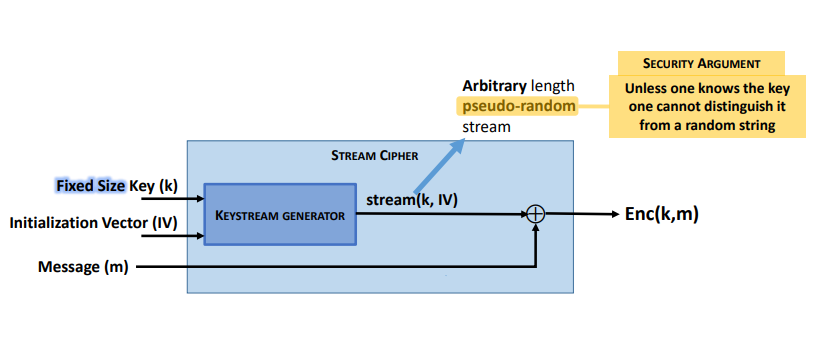
\includegraphics[scale=0.4]{screenshots/2026-10-10_1.png}
\end{center}
\end{parag}
\begin{center}
\begin{tabular}{c|c}
	(+) Speed & Algorithm are linear in time and constant in space.  \\
	\hline
	(+) Low Error Propagation & Errors in one bit do not affect subsequent symbols. \\
	\hline
	(-) Low Diffusion & A change in one plaintext bit only affects one ciphertext bit. \\
	\hline
	(-) Susceptibility to Modification & Low diffusion makes it easier to tamper with the message (like the OTP). \\
\end{tabular}
\end{center}

\begin{parag}{Cryptanalysis: The Problem with Periodicity}
    Key Stream Generators which have finite state are eventually \important{periodic}, hence if the message is longer than the period, the stream repeats which allows attacker to exploit it: if the period is identified, and too small, the key stream is known for the entire message.
\end{parag}



\subsection{Interlude on building KSG}
\begin{framedremark}
You are not expected to fully understand the following subsection, they are here to illustrate some design patterns for KSG, and challenges involved in building secure KSG, and hint at the math needed to study these objects.
\end{framedremark}
\paragraph{The linear Feedback Shift Register Building block for KSG}%
\label{par:The linear Feedback Shift Register Building block for KSG}

\begin{itemize}
    \item  \textbf{Linear Recurrence Relation}, The next output bit is a linear function (XOR) of previous bits, apply a recurrence relation to extend the initial random sequence of bits, into an arbitrary length sequence of (maybe?) randomly looking bits:
    \item For example, start with an initial state of 4 bits, $a_0, \ldots, a_3$ and 
		\begin{align*} 
			a_n =  a_{n-3} \oplus a_{n-4} 
		\end{align*}
		\item Output Sequence (starting from $1, 0, 0, 0$): $1, 0, 0, 0, 1, 0, 0, 1, 1, \ldots$
		\item \textbf{Advantage}: Uses only \textbf{shift registers} (for state storage) and \textbf{XOR gates} (for feedback), so it is extremely fast and efficient to implement in hardware.
\end{itemize}
\begin{parag}{Randomness of LFSR}
    \begin{itemize}
        \item \textbf{Maximal Period}: If the characteristic polynomial (AICC1) of the recurrence relation of the LFSR is primitive (MATH-215, Algebra 3), the maximum possible number of states before repeating: For an L-bit register, the maximum period is $2^{L}-1$ states.
    	\item \textbf{Distribution Property}: As a consequence, the sequence generated exhibit good distribution properties. Specifically, every possible nonzero state appears exactly once in the cycle, so over one full cycle of values, the output sequence are highly balanced. For example, the sequence will contain exactly $2^{L-1}$ ones and $2^{L-1}-1$ zeros. 
    \end{itemize}
\end{parag}
\begin{parag}{LFSR --- Math Danger}
    \begin{itemize}
        \item Despite passing some statistical tests, the underlying operation of an LFSR is purely \textbf{linear}
        \item \textbf{Consequence}: Techniques like the Berlekamp-Massey algorithm (beyond the scope of the class) can recover the entire LFSR state and the key stream by observing only a short segment of the output, breaking the cipher.
        \item \textbf{LFSRs should not be used directly as a Key Stream Generators}, though it has been traditionally used as a building block of Key Stream Generators
    \end{itemize}
\end{parag}

\begin{parag}{The A5/1 Cipher}
    \begin{itemize}
        \item A5/1: Used historically to secure GSM mobile phone communications.
        \item It was built by \textbf{combining multiple LFSRs} in a non-linear way to try and overcome the linearity flaw while still being cheap and having the nice statistical properties.
        \item \textbf{The Break}: despite the increased complexity, mathematical weaknesses were found, allowing the cipher to be broken much fast than brute force.
    \end{itemize}
    \begin{center}
    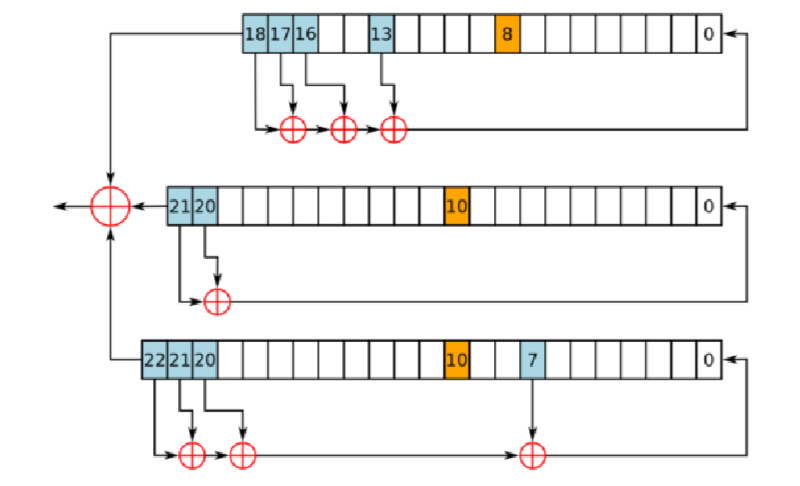
\includegraphics[scale=0.3]{screenshots/2026-10-10_2.png}
    \end{center}
\end{parag}

\begin{parag}{Non borken Stream Ciphers}
    There are alternative, modern stream ciphers for which there are no known practical cryptanalysis. Some example are \important{Trivium} (based on NLFSRs, variation of LFSRs) and \important{Salsa20} (using different techniques).
\end{parag}
\begin{figure}[htpb]
	\centering
	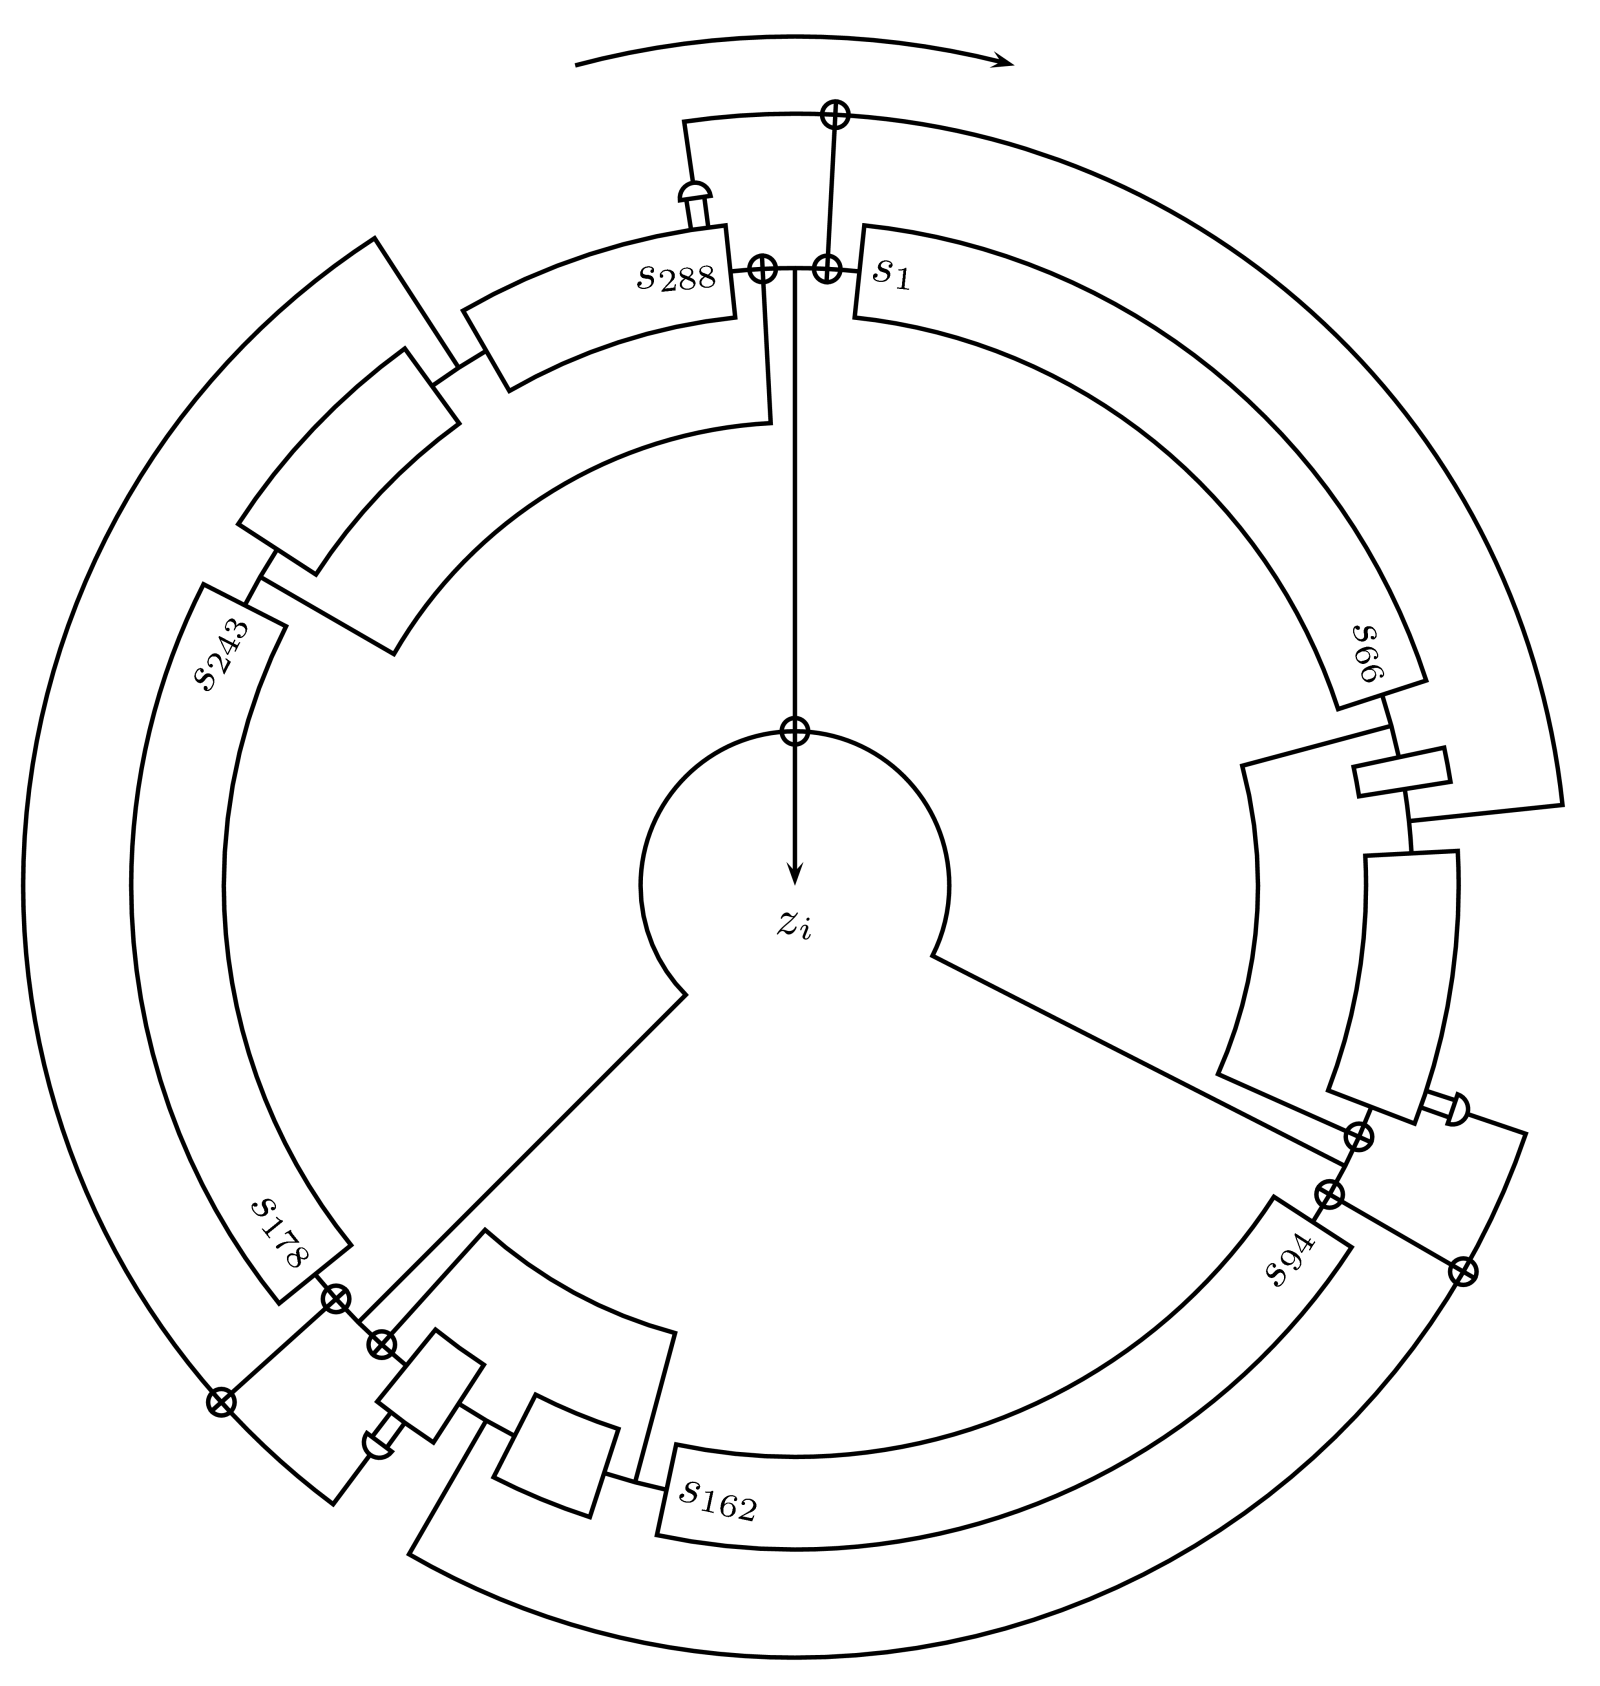
\includegraphics[scale=0.1]{screenshots/Trivium_(cipher).png}
	\caption{Structure of Trivium (Wikipedia)}
	\label{fig:}
\end{figure}
\begin{parag}{Bit Security and Consequences}
    The \important{cost of breaking}, the goal is to exploit a mathematical property or bug that can break the scheme much faster than $2^{\left|K\right|}$ attempts, which therefore \important{reduce the bit security}. As we can see the difficulty of those scheme is in the design of mathematically secure and subtly resistant primitives which has been found to be incredibly hard.
	\begin{subparag}{Best practice}
	    Use \important{well-vetted}, \important{peer-reviewed}, \important{standard algorithms and their implementation} (like AES, ChaCha20, SHA-3)
	\end{subparag}
\end{parag}





\section{Public Key Cryptography}

\begin{parag}{The Key Distribution Problem}
    As seen before, symmetric ciphers are fast, but require a pre-shared secret key. But a more fundamental question come first, if Eve can observe all conversation between Alice and Bob, how can they first agree on a secret key without having Eve to know?\\
	$ $\\
	The answer to that is public-key cryptography which allowed two parties who have never met to establish a secure channel. A famous example is Diffie-Hellman
\end{parag}
\begin{parag}{Diffie-Hellman Setup}
    Alice, Bob (and Eve) know a large public parameters: a prime number $p$ and a generator $g$
	\begin{subparag}{Alice Actions}
	    \begin{itemize}
	        \item Choose a \important{private} secret $a$
	        \item Compute the public value $A =  g^{a} \Mod p$
	        \item Sends $A$ to Bob
	    \end{itemize}
	\end{subparag}
	\begin{subparag}{Bob's Actions}
	    \begin{itemize}
	        \item Chooses a private secret $b$
	        \item Computes the Public Value $B = g^{b} \Mod p$
	        \item Sends $B$ to Alice
	    \end{itemize}
	\end{subparag}
	\begin{framedremark}
	Eve sees $A, B, g$ and $p$ but cannot find $a$ or $b$ due to the Discrete Log Problem, while it has a low complexity to compute g to the power b modulo p (with fast modular exponentiation algorithm, for example), there are no known fast (polynomial) algorithm to recover a from A and p (or b from B and p).
	\end{framedremark}
\end{parag}
\begin{parag}{The Shared Secret}
    Both Alice and Bob can compute a shared secret $K$
	\begin{align*} 
		K = B^{a} \Mod p &= \left(g^{b}\right)^{a} \Mod p\\
						 &= g^{ba} \Mod p\\
						 &= g^{ab} \Mod p\\
						 &= \left(g^{b}\right)^{a} \Mod p = A^{b} \Mod p
	\end{align*}
	Where but $B^{a} \Mod p$ and $A^{b} \Mod p$ are computable by Alice and Bob resp. However Eve cannot compute $K$ ,because she has neither $a$ nor $b$.
\end{parag}

\begin{parag}{Trapdoor Functions}
    This example of DF is one of the many examples of how to do public key cryptography to establish a shared secret (a shared key) to then do symmetric cryptography. They boil down to mathematical functions that are \important{easy to compute} in one direction but \important{hard} (high complexity) to do in the other direction. Those rely on underlying difficulty, for DH it is the \important{Discrete Logarithm Problem}.
\end{parag}
\begin{parag}{Beyond DH}
    There are other ways to set a shared secret (or even to directly communicate), all involve interesting mathematics.
	\begin{itemize}
	    \item \important{RSA}: Based on the factoring problem
	    \item \important{Elliptic Curve Cryptography (ECC)}: Can do Discrete Log on ECC, instead of on public-key crypto
	    \item \important{Post-Quantum Cryptography}: new primitives (like \important{Lattice Crypto}) to resist quantum computers.
	\end{itemize}
\end{parag}
\begin{parag}{Man In The Middle (MITM)}
    The classical version of Diffie-Hellman is vulnerable to active attack, as it only guarantees key agreement, but not authenticity (verifying who you are agreeing with). If for instance Eve intercepts $A$ from Alice and $B$ from Bob. Eve can impersonates : 
	\begin{itemize}
	    \item Eve sends $E_B$ to Alice. Alice compute $K_{AE}$
	    \item Eve Sends $E_A$ to Bob. Bob compute $K_{BE}$
	    \item Eve shares a key $K_{AE}$ with Alice and a separate key $K_{BE}$ with Bob.
	    \item She can read, modify and relay all communication.
	\end{itemize}
	Hence this implies a need for \important{trust} (authentication). DH solves the key distribution problem but create the identity verification one. The solution to this is that DH must be paired with a mechanism (like digital signature) to verify identity. The setup in this case requires a third party that needs to be trusted (a certificate authority) for public key ownership.
\end{parag}





















